\documentclass[11pt]{report}

% Paquetes y configuraciones adicionales
\usepackage{graphicx}
\usepackage[export]{adjustbox}
\usepackage{caption}
\usepackage{float}
\usepackage{titlesec}
\usepackage{geometry}
\usepackage[hidelinks]{hyperref}
\usepackage{titling}
\usepackage{titlesec}
\usepackage{parskip}
\usepackage{wasysym}
\usepackage{tikzsymbols}
\usepackage{fancyvrb}
\usepackage{xurl}
\usepackage{hyperref}
\usepackage[spanish]{babel}

\newcommand{\subtitle}[1]{
  \posttitle{
    \par\end{center}
    \begin{center}\large#1\end{center}
    \vskip0.5em}
}

% Configura los márgenes
\geometry{
  left=2cm,   % Ajusta este valor al margen izquierdo deseado
  right=2cm,  % Ajusta este valor al margen derecho deseado
  top=3cm,
  bottom=3cm,
}

% Configuración de los títulos de las secciones
\titlespacing{\section}{0pt}{\parskip}{\parskip}
\titlespacing{\subsection}{0pt}{\parskip}{\parskip}
\titlespacing{\subsubsection}{0pt}{\parskip}{\parskip}

% Redefinir el formato de los capítulos y añadir un punto después del número
\makeatletter
\renewcommand{\@makechapterhead}[1]{%
  \vspace*{0\p@} % Ajusta este valor para el espaciado deseado antes del título del capítulo
  {\parindent \z@ \raggedright \normalfont
    \ifnum \c@secnumdepth >\m@ne
        \huge\bfseries \thechapter.\ % Añade un punto después del número
    \fi
    \interlinepenalty\@M
    #1\par\nobreak
    \vspace{10pt} % Ajusta este valor para el espacio deseado después del título del capítulo
  }}
\makeatother

% Configura para que cada \chapter no comience en una pagina nueva
\makeatletter
\renewcommand\chapter{\@startsection{chapter}{0}{\z@}%
    {-3.5ex \@plus -1ex \@minus -.2ex}%
    {2.3ex \@plus.2ex}%
    {\normalfont\Large\bfseries}}
\makeatother

%==============================================================================
% Cosas para la documentación LateX
% % Sangría
% \setlength{\parindent}{1em}Texto

% % Quitar sangría
% \noindent

% % Punto
% \CIRCLE \ \ \textbf{Texto} \emph{algo}
% \begin{itemize}
%   \item \textbf{Negrita:} Texto
%   \item \textbf{Negrita:} Texto
% \end{itemize}

% % Introducir código
% \begin{center}
%   \begin{BVerbatim}
%     ... Código
%   \end{BVerbatim}
% \end{center}

% Poner una imagen
% \begin{figure}[H]
%   \centering
%   \includegraphics[scale=0.55]{img/}
%   \caption{Exportación de la base de datos en formato sql}
%   \label{fig:exportación de la base de datos en formato sql}
% \end{figure}

% % Poner una tabla
% \begin{table}[H]
%   \centering
%   \begin{tabular}{|c|c|c|c|}
%     \hline
%     \textbf{Campo 1} & \textbf{Campo 2} & \textbf{Campo 3} & \textbf{Campo 4} \\ \hline
%     Texto & Texto & Texto & Texto \\ \hline
%     Texto & Texto & Texto & Texto \\ \hline
%     Texto & Texto & Texto & Texto \\ \hline
%     Texto & Texto & Texto & Texto \\ \hline
%   \end{tabular}
%   \caption{Nombre de la tabla}
%   \label{tab:nombre de la tabla}
% \end{table}

%==============================================================================

\begin{document}

% Portada del informe
\title{Práctica 05. Índices y optimizacion de las bases de datos}
\subtitle{Adminstración y Diseño de Bases de Datos}
\author{Cheuk Kelly Ng Pante (alu0101364544@ull.edu.es)}
\date{29 de noviembre de 2023}

\maketitle

\pagestyle{empty} % Desactiva la numeración de página para el índice

% Índice
\tableofcontents

% Nueva página
\cleardoublepage

\pagestyle{plain} % Vuelve a activar la numeración de página
\setcounter{page}{1} % Reinicia el contador de página a 1

% Secciones del informe
% Capitulo 1
\chapter{Restauracion de la base de datos \emph{postgres\_air}}
Para la restauración de la base de datos se ha optado por usar la base de datos \emph{postgres\_air.backup}.
Antes de restaurar la base de datos, hay que crear la base de datos \emph{postgres\_air}, primero entramos
en la consola de postgres y luego creamos la base de datos con la siguiente sentencia:
\begin{center}
  \begin{BVerbatim}
    CREATE DATABASE postgres_air;
  \end{BVerbatim}
\end{center}

Una vez creada la base de datos, la restauramos con el siguiente comando:
\begin{center}
  \begin{BVerbatim}
    pg_restore -x --no-owner -U postgres -d postgres_air ./postgres_air.backup
  \end{BVerbatim}
\end{center}

% Capitulo 2
\chapter{Incluir sentencias SQL para la creación de los índices}
Tenemos las siguientes sentencias SQL:
\begin{figure}[H]
  \centering
  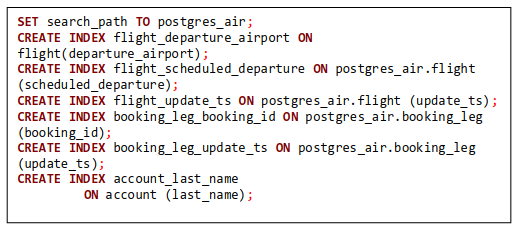
\includegraphics[scale=0.65]{img/sentencias_sql.png}
  \caption{Sentencias SQL}
  \label{fig:sentencias SQL}
\end{figure}

\chapter{Bibliografía} % En formato APA
\begin{enumerate}
\item Ng Pante, C. (2001). Titulo. Nombre pagina web. Recuperado de \url{http://url.com}

\end{enumerate}

\end{document}